\documentclass[12pt, a4paper]{article}
\usepackage[english]{babel} 
\usepackage{booktabs}
\usepackage[utf8]{inputenc} % Required for international characters
\usepackage[T1]{fontenc} % Required for output font encoding for international characters
\usepackage{tikz} % For tikz figures (to draw arrow diagrams, see a guide how to use them)
\usepackage{tikz-cd}
\usetikzlibrary{decorations.pathreplacing} % Adding libraries for decorations and paths
\usepackage{tikzsymbols} % For amazing symbols ;) https://mirror.hmc.edu/ctan/graphics/pgf/contrib/tikzsymbols/tikzsymbols.pdf 
\usepackage{geometry} % Necessary package for defining margins
\geometry{
	top=2.54cm,
	bottom=2.54cm,
	left=2.2cm,
	right=2.2cm,
}

\usepackage[backend=bibtex,style=ieee]{biblatex}
\addbibresource{ref1.bib} %this refers to the bibliography file I created
\setlength{\parindent}{15pt} % Adjust to set you indent globally 

%---------------------------------------------------------------------------------
% Define your spacing
\usepackage{setspace} % Required for spacing
\linespread{1.5}
\usepackage[T1]{fontenc} % Output font encoding for international characters
\usepackage[utf8]{inputenc} % Required for inputting international characters
\usepackage{XCharter} % Use the XCharter font
\usepackage{fancyhdr} % Package is needed to define header and footer
\pagestyle{fancy} % Allows you to customize the headers and footers
\cfoot{\footnotesize \thepage} % Define center footer


\title{Human Activity Recognition} % Adds your title
\author{
    Negar Haghbin\\
    \and
    Naghmeh Ansari\\
  }
\date{\small \today}
\begin{document}
\setcounter{page}{1} % Sets counter of page to 1
\maketitle
\thispagestyle{empty}
\section{Abstract} 
Human activity recognition (HAR) is one of the cutting-edge research topics nowadays. HAR aims to identify one’s activities based on the data gathered from wearable sensors. With this objective in mind, many classification algorithms have been used to classify human activities. These classifiers can be assessed by different evaluation methods. In this project, we are going to evaluate the performance of Decision Tree Classifier and K-Nearest Neighbors Classifier with K-Fold and Subject Cross Validation and we will show the superiority of Subject CV over K-Fold CV in HAR context. 

\section{Introduction}
In the past decades, the popularity of smart wearable devices such as smartphones, sport watches, and smart glasses had an impressive growth. This had a big impact on attracting many attentions to HAR field. Wearable HAR systems consist of a set of sensors attached to one's body in order to gather streams of data from diverse activities. HAR has many applications ranging from security to sports training and healthcare.
Due to the variety of application, different classifiers can be used which they will have different accuracy based on the dataset in use. To name some of these classifiers we can mention Decision Trees, Naive Bayes, SVM, K-Nearest Neighbors, Hidden Markov Models, and Random Forest. For evaluating the performance of these classifiers, we can use different cross-validation methods such as K-Fold CV,  Leave-One-Out CV and Subject CV. However, it is not convenient to use Leave-One-Out CV for big datasets due to its computational overhead.
\subsection{Activity Recognition Process (ARP)} 
Activity Recognition Process (ARP) is a fundamental part of HAR systems. There are 5 steps in this process: Data acquisition, Preprocessing, Segmentation, Feature Extraction, and Classification. In the first step, data is gathered through sensors attached to different body parts. These gathered data points may include artifacts that can be removed by low-pass filtering which is done in the preprocessing step. In segmentation step, data is divided into time windows. Time windows can be “overlapping”, which they have mutual data points, or “non-overlapping”, which there is no intersection between consecutive windows. Each window is labeled with the most frequent label in that time window. Window size is an important factor that heavily impacts a classifier’s performance. The optimized window size is achieved by trial and error. \cite{banos}
In feature extraction step, data points in a window are transformed into a single vector of features such as statistical moments of that time window’s columns. Finally, these vectors and their corresponding labels are given to classifiers to build the model.
\subsection{Related Works}
There are several studies that have been previously conducted in this field. Dehghani et al. \cite{dehghani}  evaluate four classifiers (K-nearest neighbor (KNN), Decision tree (DT), Naive Bayes, Nearest Centroid Classifier) through Subject CV on ARP, and indicate the superiority of it over k-fold in HAR both with overlapping and with non-overlapping sliding windows. Baños et al. \cite{banos} investigate the selection of window size for optimal classification performance. In this project, we aim to reproduce the work of \cite{dehghani}  for KNN and DT on non-overlapping time windows.

\section{Materials and Methods}
\subsection{Classifiers}
One of the classifiers that is used in this project is Decision Tree. Decision Tree Classifier repetitively divides the dataset into subsets by identifying thresholds. The algorithm terminates when the dataset is divided into classes that only contain members of a single class or some criteria of classifier attributes are met. In a decision tree, each node represents a feature, each link represents a decision or rule and each leaf represents an outcome. In our case, the outcomes are categories of activities.
The other classifier that is used in this project is K-Nearest Neighbors classifier. An object is classified by a plurality vote of its neighbors, with the object being assigned to the class most common among its k nearest neighbors. k is typically a small positive integer. In our case classes are categories of activities.

\subsection{Cross Validation}
For evaluating models, 2 cross validation methods are used: K-Fold CV and Subject CV. In K-Fold CV the dataset will be randomly partitioned to k splits with similar size and in each iteration, k-1 partitions will be used as train data and 1 partition as test data. K-Fold assumes that data points are Independent and Identically Distributed (i.i.d). This assumption does not apply to HAR dataset. First of all, in HAR context, the data that is gathered from each subject has a higher level of correlation rather than data from different subjects due to individual properties like gender, physical form, and strength. In addition, there is a small dependency between data that is gathered from one subject in a short time interval due to different moods and fatigue levels in different sessions.
These mentioned limitations may affect k-fold accuracy and result in an overestimation of a model's performance in HAR context. To address this problem, \cite{dehghani}  purposed Subject CV which in each iteration one subject is used as test data and others are used as training data. This method does not assume any correlation between subjects.

\section{Experiment}

\subsection{The Dataset}
In our project, we use the dataset gathered by Baños et al. \cite{dataset} This dataset is consists of data for 17 subjects’ activities which is gathered by 9 Xsens sensors attached to different parts of their bodies. The participants will perform 33 activities ranging from warm-up activities to fitness workouts. This dataset has 120 columns. The first two columns are the timestamps and the last column is the label for each activity. Remaining columns represent sensors’ data. Each sensor data is represented in 13 columns. Sensors gather data for acceleration, gyroscope and magnetic field in 3 directions (x, y, z) and orientation data in quaternion format.\cite{dataset} The dataset also provides data for 3 sensor displacement scenarios “ideal”, “self-placement” and “mutual-displacement”. Since \cite{dehghani}  only used acceleration data and “ideal” placement for sensors, we will also only use the same data in our project.

\subsection{Study set up}
For data preparation, Pyspark RDD data structure is used. We start by filtering “Ideal” sensor displacement data and extracting acceleration data from each subject data file. Since our baseline paper did not use any preprocessing on data we will not apply any either. Afterwards, each file is segmented to non-overlapping window sizes varying from 0.25s to 7s with 0.25s steps. For extracting each window’s feature set, mean operation is applied on its columns. Additionally, the most frequent label in each window is used as the label of that window. Following \cite{dehghani}  we used \texttt{scikit-learn 0.20.3} library for implementation. To evaluate models, we used K-Fold CV and Subject CV as in \cite{dehghani} . We used F1 score as performance criterion which is computed as shown below:

$$F1=\frac{2 \times (precision \times recall) }{precision + recall}$$

This F1-score calculation is defined by \texttt{f1-micro} scoring model in \texttt{scikit-learn} which is defined by the total number of true positives, false negatives, and false positives across all the classes.
We used the \texttt{cross\_val\_score} function of \texttt{scikit-learn} for both validations. As parameters of this function, we used \texttt{ShuffleSplit} for K-Fold CV and a customized cross-validation method for Subject CV which yields indices of train data and test data based on each subject.

\section{Results}
In this paper, we intend to reproduce the work done in \cite{dehghani} . Figure \ref{fig:kfold} shows f1-scores for K-fold CV on different non-overlapping time windows. Figure \ref{fig:kfold}.a shows the diagram for both classifiers in our project and Figure \ref{fig:kfold}.b shows the diagram taken from our baseline paper. As illustrated in our diagram, KNN has a decreasing trend from 0.96 to 0.90 with its peak at window size 0.25 and DT has a rising trend from 0.91 until it reaches a maximum point at window size 1.5. Then it has a decreasing trend until f1-score 0.86. However, in Figure 1.b we observe a decreasing trend starting for KNN from 0.96 to 0.84 peaking at time window 0.25s and for DT from 0.90 to 0.80 peaking at time window 0.25s.
Figure \ref{fig:subject} shows the diagram of Subject CV for both classifiers on different time windows. As illustrated in the diagram, KNN has almost the same decreasing trend as K-Fold in range of  0.86 to 0.82 with the peak at window size 0.25 and DT from 0.79 to 0.77 with the peak at window size 2.25. Similar diagram in \cite{dehghani}  shows a decreasing trend in the range of 0.85 to 0.77 for KNN and peak at window size of 0.25s and range of 0.79 to 0.71 and peak at window size of 1s. Although optimal window size for DT in our project is not similar to \cite{dehghani}, its difference between Subject CV and k-fold CV is the same (0.75s). These similarities led us to rely more on our results.

K-Fold CV run time for KNN was 10 minutes and for DT was 19 minutes on average. Subject CV run time for KNN was 29 minutes and for DT was 31 minutes on average. These results are gathered from running our implementation on a Mac operating system with a 2.9 GHz Intel Core i5 processor and 8GB of RAM.

\begin{figure}[htpb!] 
    \centering 
\includegraphics[scale=0.35]{figure/KFOLD.jpg} 
    \caption{Non-overlapping windowing- 10-fold CV process. a. project results. b.baseline results extracted from \cite{dehghani} .} 
    \label{fig:kfold}
\end{figure}

\begin{figure}[htpb!] 
    \centering 
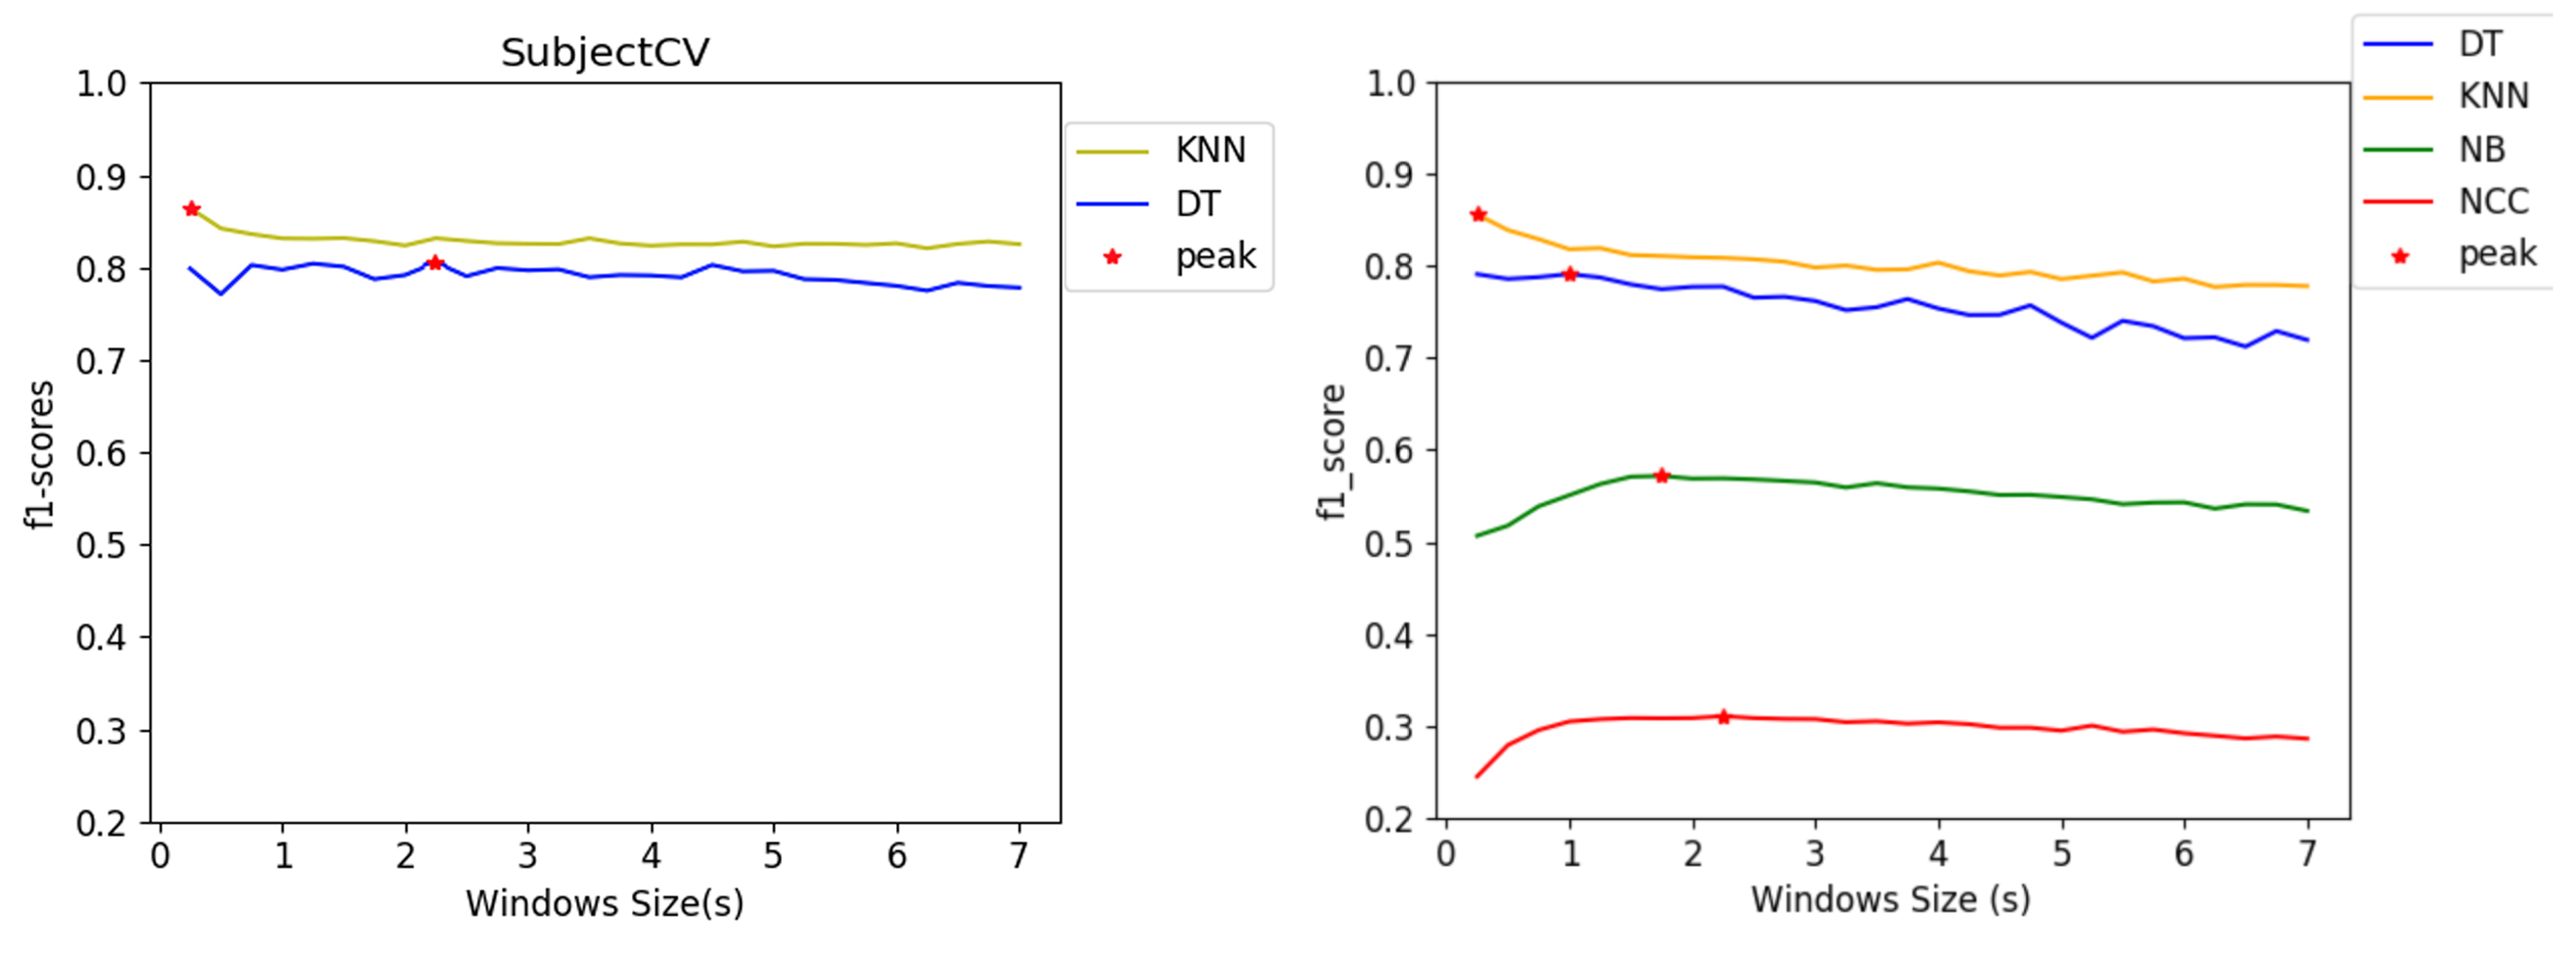
\includegraphics[scale=0.35]{figure/subject.jpg}
    \caption{Non-overlapping windowing- Subject CV process. a. project results. b.baseline results extracted from \cite{dehghani} .}
    \label{fig:subject}
\end{figure}

\section{Discussion}
By comparing figures we can see that the overall estimation of models has decreased for Subject CV. F1-score for KNN has decreased around 6.2\% and for DT there is a decrease of 6.5\%. Although the decrease is not as much as our baseline paper, it still proves that k-fold cross validation overestimates the performance of classifiers in ARP and data that is gathered from the same subject cannot be considered independent. Hence, K-Fold CV is not suggested to be used in ARP. Moreover, our results for DT classifier are less dependant on window size and we can see a less steep line comparing to baseline paper.
Additionally, the highest F1-score that is reached in Subject CV is 0.86 (KNN). This indicates that there can be improvements for this implementation and for sure use of more individuals as subjects can help classifiers to reach better f1-scores. We believe the minor differences between our results and baseline paper’s results are derived from different implementations for cross-validations. All the codes for our implementation is available in our github repository. \footnote{https://github.com/negzo/bigdataproject.git}

\subsection{Challenges}
One of the main challenges that we faced during this project was K-Fold implementation in \texttt{scikit-learn} that does not have a shuffle step that consequently misguided us for an inaccurate implementation of k-fold cross-validation.
Moreover, absence of a system with a better processor resulted in a higher run-time.

\printbibliography
\end{document}